\documentclass[tikz,border=10pt]{standalone}
\usepackage{pgfplots}
\pgfplotsset{compat=1.18}
\begin{document}
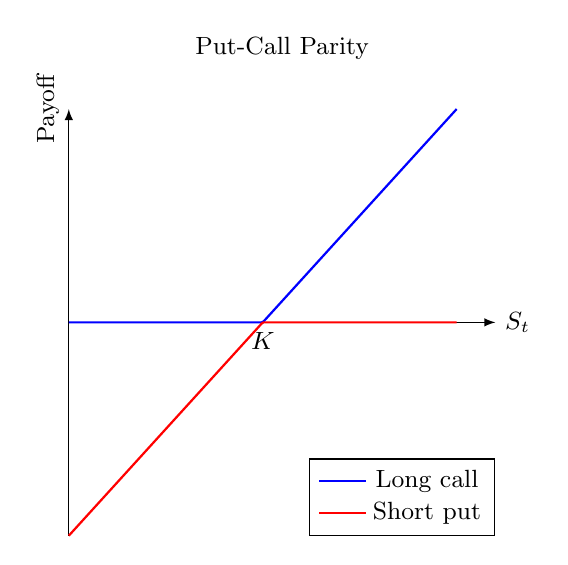
\begin{tikzpicture}[font=\small]
  \pgfmathsetmacro{\K}{1}        % strike price
  \begin{axis}[
      width=7cm, height=7cm,
      axis x line=middle,
      axis y line=left,
      axis line style={-latex},
      xmin=0, xmax=2.2,
      ymin=-1, ymax=1,
      xtick=\empty, ytick=\empty,
      domain=0:2,
      samples=200,
      clip=false,
      xlabel={$S_t$},
      xlabel style={at={(axis description cs:1,0.5)}, anchor=west},
      ylabel={Payoff},
      ylabel style={at={(axis description cs:0,1)}, anchor=south},
      title style={
          at={(axis description cs:0.5,1)},
          yshift=0.3cm,
          anchor=south,
        },
      title={Put-Call Parity},
      legend style={at={(axis description cs:1,0)}, anchor=south east},
    ]

    \addplot[blue, solid, thick] {max(x-\K,0)}; \addlegendentry{Long call}
    \addplot[red, solid, thick] {-max(\K-x,0)}; \addlegendentry{Short put}

    \node[below] at (axis cs:\K,0) {$K$};

  \end{axis}
\end{tikzpicture}
\end{document}